\documentclass[tikz,border=4pt]{standalone}
\usepackage[T1]{fontenc}
\usepackage[utf8]{inputenc}
\usepackage{amsmath,amssymb}
\usepackage{helvet}
\renewcommand{\familydefault}{\sfdefault}
\usepackage{pgfplots}
\pgfplotsset{compat=1.17}
\usetikzlibrary{arrows.meta,positioning,calc,fit,backgrounds,shapes.geometric}

\definecolor{cVis}{HTML}{1F77B4}
\definecolor{cTxt}{HTML}{D62728}
\definecolor{cProj}{HTML}{2CA02C}
\definecolor{cLLM}{HTML}{9467BD}
\definecolor{cConv}{HTML}{FF7F0E}
\definecolor{cAtt}{HTML}{17BECF}
\definecolor{cGray}{HTML}{7F7F7F}

\tikzset{
  blk/.style={draw, rounded corners=2pt, minimum height=8mm, align=center, font=\footnotesize, thick},
  tok/.style={draw, minimum size=3.2mm, inner sep=0pt},
  arr/.style={-{Stealth[length=2mm]}, thick},
}

\begin{document}
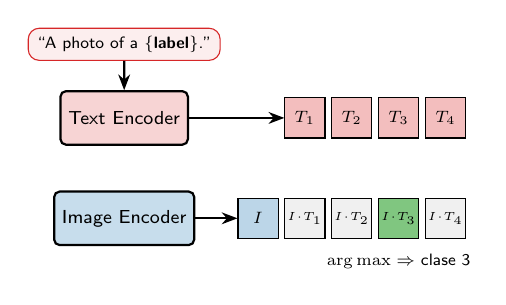
\begin{tikzpicture}[scale=.85, every node/.style={transform shape}]
  \node[font=\scriptsize, align=left, draw=cTxt, rounded corners, fill=cTxt!8] (p) at (0,2.2) {``A photo of a \{\textbf{label}\}.''};
  \node[blk, fill=cTxt!20] (te) at (0,1.1) {Text Encoder};
  \draw[arr] (p) -- (te);
  \foreach \j in {1,...,4}{\node[tok,fill=cTxt!30,minimum size=6mm] (T\j) at (2.0+\j*0.7,1.1) {\scriptsize$T_\j$};}
  \draw[arr] (te) -- (T1);
  \node[blk, fill=cVis!25] (ie) at (0,-0.4) {Image Encoder};
  \node[tok,fill=cVis!30,minimum size=6mm] (I1) at (2.0,-0.4) {\scriptsize$I$};
  \draw[arr] (ie) -- (I1);
  \foreach \j in {1,...,4}{\ifnum\j=3 \def\cc{cProj!60}\else\def\cc{black!6}\fi\node[tok,fill=\cc,minimum size=6mm] at (2.0+\j*0.7,-0.4) {\tiny$I\!\cdot\!T_\j$};}
  \node[font=\scriptsize] at (4.1,-1.05) {$\arg\max \Rightarrow$ clase 3};
\end{tikzpicture}
\end{document}
